\documentclass[aspectratio=169]{beamer}

\usetheme[secheader]{Boadilla}
\usecolortheme{crane}
\usepackage[latin1]{inputenc}
\usepackage{listings}

\title{Open Source Android Development Tools}
\author{Manfred Moser}
\date{July, 2011}
\institute{simpligility.com}

% \institute{simpligility technologies inc.\\[\medskipamount]
%       
\includegraphics[scale=0.6]{simpligility.png}%
% }

\logo{
\includegraphics[scale=0.25]{simpligility.png}}
\newcommand{\surl}[1] {{\tiny \url{#1}}}

\begin{document}

\begin{frame}
  \titlepage
\end{frame}

\begin{frame}{Table of Contents}
  Open Source Android Development Tools - SDK, ADT and beyond
  \setcounter{tocdepth}{1}
  \tableofcontents
\end{frame}

\begin{frame}{About Manfred}
  \begin{itemize}
    \item<1-> Android application developer
    \item<2-> Core committer Maven Android Plugin
    \item<3-> Project Owner ksoap2-android
    \item<4-> Committer RoboGuice
    \item<5-> Committer Hudson
  \end{itemize}

\end{frame}


\section{Android Itself}

  \subsection{Components}
    \begin{frame}{What components make up Android codebase?}
      \begin{description}
        \item<1->[Android Proper] \hfill \\ as found on your device
        \item<2->[Android Open Source Project AOSP] \hfill  \\ subset of above 
        \item<3->[Android Software Development Kit SDK] \hfill  \\ for Java based development applications
        \item<4->[Android Native Development Kit NDK] \hfill  \\ for C/C++ based development
        \item<5->[Android Open Accessory Development Kit ADK] \hfill \\ for USB based hardware hacking
        \item<6->[Android Development Toolkit ADT] \hfill  \\ Eclipse plugin for Android development  
      \end{description}
    \end{frame}

  \subsection{Android Proper}
    \begin{frame}{Android Proper - As Found on Your Device}
      \begin{itemize}
        \item<1->Linux
        \item<2->Apache Harmony 
        \item<3->Lots of other open source components
        \item<4->Custom Android related components like Dalvik VM
        \item<5->binary device driver and other blobs 
        \item<6->patched components, custom drivers and different applications from manufacturer and provider
      \end{itemize}
    \end{frame}
  
  \subsection{AOSP}
    \begin{frame}{Android Open Source Project AOSP}
      \begin{itemize}
        \item<1->Linux, Apache Harmony, OpenGL ES and lots more
        \item<2->numerous specific components e.g. Dalvik
        \item<3->various forks from upstream project
        \item<4->base for custom roms and such
        \item<5->various different open source licenses
        \item<6->source released in drops, sometimes late or not yet
      \end{itemize}
    \end{frame}

  \subsection{Android Tools}
    \begin{frame}{Android Tools}
      \begin{itemize}
        \item<1->development tools like ADT, DDMS and related tools that form SDK 
        \item<2->cooperating with Eclipse projects, external contributors ...
        \item<3->fully open source, all commits right to public git repo
        \item<4->available at \surl{http://tools.android.com/}
      \end{itemize}
    \end{frame}

\section{Development Tools}

  \subsection{IDEs}

    \begin{frame}{Eclipse and ADT and friends}
        \begin{itemize}
          \item<1-> default supported development environment 
          \item<2-> full tool suite including debugging, profiling and so on
          \item<3-> graphical layout editor
          \item<4-> very powerful also with help of further Eclipse plugins (e.g. Mylyn, egit\dots)
          \item<5-> well architected so that most components work outside Eclipse too
        \end{itemize}
    \end{frame}

    \begin{frame}{Other IDE's}
      \begin{description}
        \item<1->[Motorola MOTODEV Studio \surl{http://developer.motorola.com/docstools/motodevstudio/}] \hfill \\  partly open source, commiting upstream to ADT and Eclipse Sequoyah \surl{http://eclipse.org/sequoyah/} 
        \item<2->[Jetbrains IntelliJ IDEA CE \surl{http://www.jetbrains.org/}] \hfill \\ fully open source, includes Android support 
        \item<3->[Oracle Netbeans \surl{http://kenai.com/projects/nbandroid/}] \hfill \\ fully open source, community maintained plugin for Android 
        \item<4->[Emacs \surl{http://gitorious.org/emacs-android-minor-mode}] \hfill \\ fully open source, limited
      \end{description}
    \end{frame}

  \subsection{Build Tools}

    \begin{frame}{Maven Android Plugin and Friends}
      \begin{description}
       \item<1->[Maven Android Plugin \surl{http://code.google.com/p/maven-android-plugin/}] \hfill \\ build apk, deploy to devices, run tests and lots more
       \item<2->[Maven Android SDK Deployer \surl{https://github.com/mosabua/maven-android-sdk-deployer}] \hfill \\ deploy artifacts from SDK to Maven repository
       \item<3->[Android4Maven \surl{http://sourceforge.net/projects/android4maven/}] \hfill \\ bundle android.jar from AOSP to submit to Maven central
       \item<4->[M2E Android \surl{https://github.com/rgladwell/m2e-android}] \hfill \\ Maven build to play nice with ADT
       \item<5->[AndroidSDKFido \surl{https://github.com/joakime/android-sdkfido}] \hfill \\  build source and javadoc artifacts
       \item<6->[Android RIndirect \surl{https://github.com/akquinet/android-rindirect}] \hfill \\  help with component reuse
      \end{description}
    \end{frame}

    \begin{frame}{Others}
      \begin{description}
        \item<1->[Gradle Android Plugin] \surl{https://code.google.com/p/gradle-android-plugin/} \hfill \\ for the Groovy based build system Gradle
    for    \item<2->[SBT Android Plugin] \surl{https://github.com/jberkel/android-plugin} \hfill \\ for the Scala based build system SBT, Scala based Android applications
        \item<3->[Rake/Ruboto/Maven] for JRuby Android applications 
      \end{description}
    \end{frame}

    \begin{frame}{Maven Android Plugin - Example}
      \begin{itemize}
        \item<1-> deploy to multiple devices and run tests
        \item<2-> reuse of other Maven plugins
        \item<3-> use of libraries and Android components easy
        \item<4-> full release cycle sign, zipalign, automatic versioning, \dots
        \item<5-> Proguard support
        \item<6-> Native components and libraries
        \item<7-> Scala support
        \item<8-> more
      \end{itemize}
    \end{frame}

  \subsection{Other Development Tools}

    \begin{frame}{Other Development Tools}
      \begin{description}
        \item<1->[Droid at Screen \surl{http://blog.ribomation.com/2010/01/droidscreen/}] \hfill \\ device screen recorder/projector 

        \item<2->[DroidDraw \surl{http://www.droiddraw.org/}] \hfill \\  UI build and design tool 
 
        \item<3->[dex2jar \surl{http://code.google.com/p/dex2jar/}] \hfill \\ converter from dex to jar format 

        \item<4->[smali/baksmali \surl{http://code.google.com/p/smali/}] \hfill \\ dex assembler/disassembler 

        \item<5->[Android2PO \surl{https://github.com/miracle2k/android2po}] \hfill \\ Converter for Android strings to gettext 
      \end{description}
   \end{frame}

\section{Development Libraries}

  \subsection{Java Libraries}

    \begin{frame}{Java Libraries suitable for Android}
      \begin{description}
        \item<1->[Jackson \surl{http://jackson.codehaus.org/}] \hfill \\ JSON library 
        \item<2->[google-gson \surl{http://code.google.com/p/google-gson/}] \hfill \\ JSON library
        \item<3->[SimpleXML \surl{http://simple.sourceforge.net/home.php}] \hfill \\ XML serialization framework 
        \item<4->[ksoap2-android  \surl{http://code.google.com/p/ksoap2-android/}] \hfill \\ SOAP library 
        \item<5->[WSDL2Android \surl{https://github.com/kigero/WSDL2Android}] \hfill \\ code generator for ksoap2-android
        \item<6->[ormlite \surl{http://ormlite.com/}] \hfill \\ light-weight object relational mapping tool 
        \item<7->[Twitter4J] \surl{http://twitter4j.org/} \hfill \\ twitter integration library 
      \end{description}
    \end{frame}

  \subsection{Android Specific Frameworks and Libraries}

    \begin{frame}{Frameworks for General Purpose Usage}
      \begin{description}
        \item<1->[Roboguice \surl{http://roboguice.org}] \hfill \\ Google Guice IoC based framework  
        \item<2->[AndroidAnnotations \surl{http://code.google.com/p/androidannotations/}] \hfill \\ annotation based code generation framework
        \item<3->[DroidFu \surl{http://github.com/kaeppler/droid-fu}] \hfill \\ general purpose collection of helper classes
        \item<4->[CommonsWare Android Components CWAC \surl{https://github.com/commonsguy}] collection of helper classes and widget
        \item<5->[DroidKit \surl{https://github.com/droidkit/droidkit}] \hfill \\ collection of Android API extensions
        \item<6->[Libs for Android \surl{http://code.google.com/p/libs-for-android/}] \hfill \\ collection of libraries
        \item<7->[AndroidLibs \surl{http://www.androidlibs.com/}] \hfill \\ social and contact related libraries
        \item<8->[AndroidAsync \surl{https://bitbucket.org/hal/android-async/}] \hfill \\ alternate implementation for asynchronous tasks  
      \end{description}
    \end{frame}
  
  \begin{frame}{Libraries for Specific Use Cases}
      \begin{description}
        \item<1->[ZXing \surl{http://code.google.com/p/zxing/}] \hfill \\ barcode scanning library and application
        \item<2->[Jon's Java Imaging Library \surl{http://code.google.com/p/jjil/}] \hfill \\ image processing library
        \item<3->[OpenCV-Android \surl{http://billmccord.github.com/OpenCV-Android/}] \hfill \\ real time computer vision library
        \item<4->[Facebook Android SDK \surl{https://github.com/facebook/facebook-android-sdk}] \hfill \\ your guess ;-)
        \item<5->[MapsForge \surl{http://code.google.com/p/mapsforge/}] \hfill \\ OpenStreetMap toolbox
        \item<6->[OSMDroid \surl{http://code.google.com/p/osmdroid/}] \hfill \\ OpenStreetMap toolbox
      \end{description}
    \end{frame}

    \begin{frame}{Example RoboGuice}
      \begin{columns}[t]
        \begin{column}{0.2\textwidth}
          \begin{center}
            
\includegraphics[height=1.0in]{roboguice.png}
          \end{center}
        \end{column}

       \begin{column}{0.8\textwidth}
Compare yourself:

\verb|class AndroidShowCase extends Activity
%   private TextView name; 
%   public void onCreate(Bundle savedInstanceState) { 
%     super.onCreate(savedInstanceState); 
%     setContentView(R.layout.androidshowcase); 
%     name = findViewById(R.id.name);
%|
%\begin{verbatim*}
% test
%\end{verbatim*}

%  
% class AndroidShowCase extends Activity { 
%   private TextView name; 
%   public void onCreate(Bundle savedInstanceState) { 
%     super.onCreate(savedInstanceState); 
%     setContentView(R.layout.androidshowcase); 
%     name = findViewById(R.id.name);



        \end{column}
      \end{columns}
    \end{frame}
  
    \begin{frame}{UI Libraries and Widgets}
      \begin{description}
        \item<1->[GreenDroid \surl{https://github.com/cyrilmottier/GreenDroid}] \hfill \\ application framework and UI widget collection
        \item<2->[svg-android \surl{http://code.google.com/p/svg-android/}] \hfill \\ SVG rendering library
        \item<3->[View Flow for Android \surl{https://github.com/pakerfeldt/android-viewflow}] \hfill \\ horizontally scrolling views
        \item<4->[Android Wheel \surl{http://code.google.com/p/android-wheel/}] \hfill \\ wheel input control widget
        \item<5->[ActionBarSherlock \surl{http://actionbarsherlock.com/}]  \hfill \\ ActionBar support for tablets and phones
        \item<6->[Android Actionbar \surl{https://github.com/johannilsson/android-actionbar}] \hfill \\ ActionBar support for tablets and phones
      \end{description}
    \end{frame}

    \begin{frame}{More UI Libraries and Widgets}
      \begin{description}        
        \item<1->[Pull to Refresh for Android \surl{https://github.com/johannilsson/android-pulltorefresh}] \hfill \\ list refresh widget
        \item<2->[Android ColorPickerPreference \surl{https://github.com/attenzione/android-ColorPickerPreference}] \hfill \\ color picker
        \item<3->[Android AutoFitTextView \surl{https://github.com/grantland/android-autofittextview}] \hfill \\ dynamic font resizing in text view
        \item<4->[Android TextView Multiline Ellipse \surl{http://code.google.com/p/android-textview-multiline-ellipse/}] ellipse for multiline text view
        \item<5->[Android MapViewBalloons \surl{https://github.com/jgilfelt/android-mapviewballoons}] \hfill \\ UI widget for maps
      \end{description}
    \end{frame}

%     \begin{frame}{AndroidSherlock}
%       \begin{center}
%       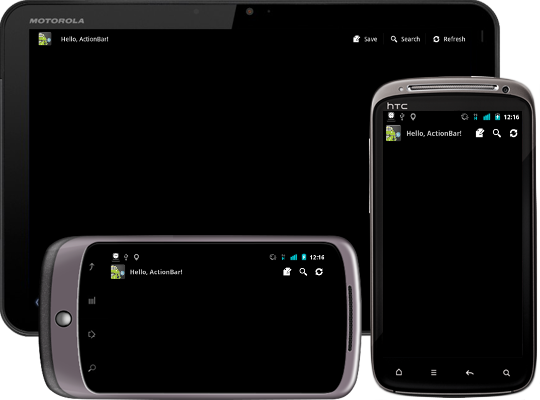
\includegraphics[height=2.5in]{androidsherlock.png}
%       \end{center}
%     \end{frame}

\subsection{Game Development Libraries}

    \begin{frame}{Game Development Libraries}
      \begin{description}
        \item<1->[libgdx \surl{http://libgdx.badlogicgames.com/}] \hfill \\ cross-platform 2D and 3D game development framework for Java/C/C++. 
        \item<2->[AndEngine \surl{http://www.andengine.org/}] \hfill \\ Java based 2D OpenGL Game Engine for Android
        \item<3->[forget3D \surl{http://code.google.com/p/forget3d/}] \hfill \\ OpenGL ES framework for Android, Win32, WinCE
        \item<4->[min3d \surl{http://code.google.com/p/min3d/}] \hfill \\ lightweight 3d library/framework for Android using Java with OpenGL ES 
        \item<5->[Angle  \surl{http://code.google.com/p/angle/}] \hfill \\ game library for 2D games using OpenGL ES
      \end{description}
    \end{frame}

  \subsection{Android Testing Tools}

    \begin{frame}{Android Testing Tools}
      \begin{description}
        \item<1->[Robotium \surl{http://robotium.org}] \hfill \\ \emph{Selenium} for Android
        \item<2->[Robolectric \surl{http://robolectric.org}] \hfill \\ Android tests run on JVM
        \item<3->[Calculon \surl{https://github.com/kaeppler/calculon}] \hfill \\ Android testing DSL
        \item<4->[Android JUnit Report \surl{https://github.com/jsankey/android-junit-report}] \hfill \\ tool to load test report from device/emulator
        \item<5->[Memory Sucker \surl{https://github.com/nollbit/memory-sucker}] \hfill \\ test tool to simulate low memory scenarios 
        \item<6->[Android Mock \surl{http://code.google.com/p/android-mock/}] \hfill \\ object mocking library
      \end{description}
    \end{frame}

    \begin{frame}{Testing Demo}
      \begin{columns}[t]
        \begin{column}[c]{0.5\textwidth}
          Robotium on DalvikVM
        \end{column}
        \begin{column}[c]{0.5\textwidth}
          Robolectric on JVM
        \end{column}
      \end{columns}
    \end{frame}

  \subsection{Others of interest}  

    \begin{frame}{Others of interest}
      \begin{description}
        \item<1->[OpenIntents \surl{http://code.google.com/p/openintents/}] \hfill \\ collection of reusable components and applications
        \item<2->[i-jetty \surl{http://code.google.com/p/i-jetty/}] \hfill \\ servlet container running on the device 
        \item<3->[Android Screenshot library \surl{http://code.google.com/p/android-screenshot-library/}] \hfill \\  programmatically take screenshots, n no root required 
        \item<4->[Android Alarm Database \surl{http://code.google.com/p/android-alarm-database/}] \hfill \\ alarm application and toolkit 
        \item<5->[Application Crash Report for Android ACRA \surl{http://code.google.com/p/acra/}] \hfill \\ crash report library
        \item<6->[Android Error Reporter \surl{https://github.com/tomquist/Android-Error-Reporter}] \hfill \\ error report library
      \end{description}
    \end{frame}

  \subsection{Other Languages}
    \begin{frame}{Other Languages}
      Java is the main language for development and API but also possible are 
      \begin{itemize}
      \item C/C++ (via NDK first class)
      \item JRuby
      \item Scala
      \item JavaScript (e.g. via PhoneGap)
      \item Processing \surl{http://wiki.processing.org/w/Android}
      \item C\#
      \end{itemize}
    \end{frame}

    \begin{frame}{Example - Scala libraries}
      \begin{itemize}
       \item Baitha \surl{https://github.com/sattvik/baitha}
       \item Positronic Net \surl{https://github.com/rst/positronic_net}
       \item Borachio mocking library \surl{http://borachio.com/}
      \end{itemize}
    \end{frame}

\section{Conclusions}

  \subsection{Android = Java?}
    \begin{frame}{Is Android Java?}
      \begin{itemize}
      \item<1-> Yes - default application programming language
      \item<2-> Yes - API is Java based
      \item<3-> No - not using a standard compliant Java Virtual Machine Runtime
      \item<4-> No - only using parts of the standard class libraries and 
      \end{itemize}
    \end{frame}

  \subsection{Android = Open Source?}
    \begin{frame}{Is Android Open Source?}
      \begin{itemize}
       \item<1-> Yes, in time - AOSP open sourced in drops
       \item<2-> Yes -ADT fully open source
       \item<3-> Yes and no - cooperation with upstream projects patchy but exists
       \item<4-> No - binary blobs for drivers and other parts
      \end{itemize}
    \end{frame}

  \subsection{Android part of Java Community?}
    \begin{frame}{Android part of the Java Community?}
     \begin{itemize}
      \item<1-> Yes - parts of Android itself
      \item<2-> Yes - tooling around Android
      \item<3-> Yes - lots of libraries and tooling from rest of Java universe
      \item<4-> Yes - lots of people from Java community, also part of Android community
      \item<5-> Yes - lots of JVM related aspects as well e.g. Scala, JRuby, Processing, Groovy...
      \end{itemize}
    \end{frame}
  
  \subsection{Android part of Open Source Community?}
    \begin{frame}{Android part of Open Source Community?}
     \begin{itemize}
      \item<1-> Yes - part of Apache Community
      \item<2-> Yes - part of Eclipse Community
      \item<3-> Yes - part of Ruby, Scala, Groovy/Gradle...
      \item<4-> Yes - lots of open source libraries specifically to Android
      \item<5-> Yes - lots of projects on Github, Google Code, ...
      \item<6-> Yes - move towards Maker community with ADK
     \end{itemize}
    \end{frame}

  \subsection{Overall Conclusions}
    \begin{frame}{Overall conclusion}
      \begin{itemize}
        \item<1-> Despite lots of flaws and kinks that make things interesting
        \item<2-> Android is part of the Java and Open Source communities
        \item<3-> Android touches a lot of other communities and brings them together
        \item<4-> Android is a great chance to collaborate and learn
      \end{itemize}
    \end{frame}

  \subsection{What can you do?}
    \begin{frame}{What can you do?}
      \begin{itemize}
        \item<1-> Buy an unlocked/unlockable device
        \item<2-> Use a custom ROM
        \item<3-> Ask for open source drops of AOSP 
        \item<4-> Encourage patches to upstream projects and 
        \item<5-> Ask for open sourcing of any closed parts, tools...
        \item<6-> Contribute and cooperate yourself! 
      \end{itemize}
    \end{frame}
\end{document}